
\documentclass[letterpaper,hide notes,xcolor={table,svgnames},pdftex,10pt]{beamer}
\def\showexamples{t}


%\usepackage[svgnames]{xcolor}

%% Demo talk
%\documentclass[letterpaper,notes=show]{beamer}

\usecolortheme{crane}
\setbeamertemplate{navigation symbols}{}

\usetheme{MyPittsburgh}
%\usetheme{Frankfurt}

%\usepackage{tipa}

\usepackage{hyperref}
\usepackage{graphicx,xspace}
\usepackage[normalem]{ulem}
\usepackage{multicol}

\newcommand\SF[1]{$\bigstar$\footnote{SF: #1}}

\usepackage[default]{sourcesanspro}
\usepackage[T1]{fontenc}

\newcounter{tmpnumSlide}
\newcounter{tmpnumNote}

% old question code
%\newcommand\question[1]{{$\bigstar$ \small \onlySlide{2}{#1}}}
% \newcommand\nquestion[1]{\ifdefined \presentationonly \textcircled{?} \fi \note{\par{\Large \textbf{?}} #1}}
% \newcommand\nanswer[1]{\note{\par{\Large \textbf{A}} #1}}


 \newcommand\mnote[1]{%
   \addtocounter{tmpnumSlide}{1}
   \ifdefined\showcues {~\tiny\fbox{\arabic{tmpnumSlide}}}\fi
   \note{\setlength{\parskip}{1ex}\addtocounter{tmpnumNote}{1}\textbf{\Large \arabic{tmpnumNote}:} {#1\par}}}

\newcommand\mmnote[1]{\note{\setlength{\parskip}{1ex}#1\par}}

%\newcommand\mnote[2][]{\ifdefined\handoutwithnotes {~\tiny\fbox{#1}}\fi
% \note{\setlength{\parskip}{1ex}\textbf{\Large #1:} #2\par}}

%\newcommand\mnote[2][]{{\tiny\fbox{#1}} \note{\setlength{\parskip}{1ex}\textbf{\Large #1:} #2\par}}

\newcommand\mquestion[2]{{~\color{red}\fbox{?}}\note{\setlength{\parskip}{1ex}\par{\Large \textbf{?}} #1} \note{\setlength{\parskip}{1ex}\par{\Large \textbf{A}} #2\par}\ifdefined \presentationonly \pause \fi}

\newcommand\blackboard[1]{%
\ifdefined   \showblackboard
  {#1}
  \else {\begin{center} \fbox{\colorbox{blue!30}{%
         \begin{minipage}{.95\linewidth}%
           \hspace{\stretch{1}} Some space intentionally left blank; done at the blackboard.%
         \end{minipage}}}\end{center}}%
         \fi%
}



%\newcommand\q{\tikz \node[thick,color=black,shape=circle]{?};}
%\newcommand\q{\ifdefined \presentationonly \textcircled{?} \fi}

\usepackage{listings}
\lstset{%
  keywordstyle=\bfseries,
  aboveskip=15pt,
  belowskip=15pt,
  captionpos=b,
  identifierstyle=\ttfamily,
  escapeinside={(*@}{@*)},
  stringstyle=\ttfamiliy,
  frame=lines,
  numbers=left, basicstyle=\scriptsize, numberstyle=\tiny, stepnumber=0, numbersep=2pt}

\usepackage{siunitx}
\newcommand\sius[1]{\num[group-separator = {,}]{#1}\si{\micro\second}}
\newcommand\sims[1]{\num[group-separator = {,}]{#1}\si{\milli\second}}
\newcommand\sins[1]{\num[group-separator = {,}]{#1}\si{\nano\second}}
\sisetup{group-separator = {,}, group-digits = true}

%% -------------------- tikz --------------------
\usepackage{tikz}
\usetikzlibrary{positioning}
\usetikzlibrary{arrows,backgrounds,automata,decorations.shapes,decorations.pathmorphing,decorations.markings,decorations.text}

\tikzstyle{place}=[circle,draw=blue!50,fill=blue!20,thick, inner sep=0pt,minimum size=6mm]
\tikzstyle{transition}=[rectangle,draw=black!50,fill=black!20,thick, inner sep=0pt,minimum size=4mm]

\tikzstyle{block}=[rectangle,draw=black, thick, inner sep=5pt]
\tikzstyle{bullet}=[circle,draw=black, fill=black, thin, inner sep=2pt]

\tikzstyle{pre}=[<-,shorten <=1pt,>=stealth',semithick]
\tikzstyle{post}=[->,shorten >=1pt,>=stealth',semithick]
\tikzstyle{bi}=[<->,shorten >=1pt,shorten <=1pt, >=stealth',semithick]

\tikzstyle{mut}=[-,>=stealth',semithick]

\tikzstyle{treereset}=[dashed,->, shorten >=1pt,>=stealth',thin]

\usepackage{ifmtarg}
\usepackage{xifthen}
\makeatletter
% new counter to now which frame it is within the sequence
\newcounter{multiframecounter}
% initialize buffer for previously used frame title
\gdef\lastframetitle{\textit{undefined}}
% new environment for a multi-frame
\newenvironment{multiframe}[1][]{%
\ifthenelse{\isempty{#1}}{%
% if no frame title was set via optional parameter,
% only increase sequence counter by 1
\addtocounter{multiframecounter}{1}%
}{%
% new frame title has been provided, thus
% reset sequence counter to 1 and buffer frame title for later use
\setcounter{multiframecounter}{1}%
\gdef\lastframetitle{#1}%
}%
% start conventional frame environment and
% automatically set frame title followed by sequence counter
\begin{frame}%
\frametitle{\lastframetitle~{\normalfont(\arabic{multiframecounter})}}%
}{%
\end{frame}%
}
\makeatother

\makeatletter
\newdimen\tu@tmpa%
\newdimen\ydiffl%
\newdimen\xdiffl%
\newcommand\ydiff[2]{%
    \coordinate (tmpnamea) at (#1);%
    \coordinate (tmpnameb) at (#2);%
    \pgfextracty{\tu@tmpa}{\pgfpointanchor{tmpnamea}{center}}%
    \pgfextracty{\ydiffl}{\pgfpointanchor{tmpnameb}{center}}%
    \advance\ydiffl by -\tu@tmpa%
}
\newcommand\xdiff[2]{%
    \coordinate (tmpnamea) at (#1);%
    \coordinate (tmpnameb) at (#2);%
    \pgfextractx{\tu@tmpa}{\pgfpointanchor{tmpnamea}{center}}%
    \pgfextractx{\xdiffl}{\pgfpointanchor{tmpnameb}{center}}%
    \advance\xdiffl by -\tu@tmpa%
}
\makeatother
\newcommand{\copyrightbox}[3][r]{%
\begin{tikzpicture}%
\node[inner sep=0pt,minimum size=2em](ciimage){#2};
\usefont{OT1}{phv}{n}{n}\fontsize{4}{4}\selectfont
\ydiff{ciimage.south}{ciimage.north}
\xdiff{ciimage.west}{ciimage.east}
\ifthenelse{\equal{#1}{r}}{%
\node[inner sep=0pt,right=1ex of ciimage.south east,anchor=north west,rotate=90]%
{\raggedleft\color{black!50}\parbox{\the\ydiffl}{\raggedright{}#3}};%
}{%
\ifthenelse{\equal{#1}{l}}{%
\node[inner sep=0pt,right=1ex of ciimage.south west,anchor=south west,rotate=90]%
{\raggedleft\color{black!50}\parbox{\the\ydiffl}{\raggedright{}#3}};%
}{%
\node[inner sep=0pt,below=1ex of ciimage.south west,anchor=north west]%
{\raggedleft\color{black!50}\parbox{\the\xdiffl}{\raggedright{}#3}};%
}
}
\end{tikzpicture}
}


%% --------------------

%\usepackage[excludeor]{everyhook}
%\PushPreHook{par}{\setbox0=\lastbox\llap{MUH}}\box0}

%\vspace*{\stretch{1}

%\setbox0=\lastbox \llap{\textbullet\enskip}\box0}

\setlength{\parskip}{\fill}

\newcommand\noskips{\setlength{\parskip}{1ex}}
\newcommand\doskips{\setlength{\parskip}{\fill}}

\newcommand\xx{\par\vspace*{\stretch{1}}\par}
\newcommand\xxs{\par\vspace*{2ex}\par}
\newcommand\tuple[1]{\langle #1 \rangle}
\newcommand\code[1]{{\sf \footnotesize #1}}
\newcommand\ex[1]{\uline{Example:} \ifdefined \presentationonly \pause \fi
  \ifdefined\showexamples#1\xspace\else{\uline{\hspace*{2cm}}}\fi}

\newcommand\ceil[1]{\lceil #1 \rceil}


\AtBeginSection[]
{
   \begin{frame}
       \frametitle{Outline}
       \tableofcontents[currentsection]
   \end{frame}
}



\pgfdeclarelayer{edgelayer}
\pgfdeclarelayer{nodelayer}
\pgfsetlayers{edgelayer,nodelayer,main}

\tikzstyle{none}=[inner sep=0pt]
\tikzstyle{rn}=[circle,fill=Red,draw=Black,line width=0.8 pt]
\tikzstyle{gn}=[circle,fill=Lime,draw=Black,line width=0.8 pt]
\tikzstyle{yn}=[circle,fill=Yellow,draw=Black,line width=0.8 pt]
\tikzstyle{empty}=[circle,fill=White,draw=Black]
\tikzstyle{bw} = [rectangle, draw, fill=blue!20, 
    text width=4em, text centered, rounded corners, minimum height=2em]
    
    \newcommand{\CcNote}[1]{% longname
	This work is licensed under the \textit{Creative Commons #1 3.0 License}.%
}
\newcommand{\CcImageBy}[1]{%
	\includegraphics[scale=#1]{creative_commons/cc_by_30.pdf}%
}
\newcommand{\CcImageSa}[1]{%
	\includegraphics[scale=#1]{creative_commons/cc_sa_30.pdf}%
}
\newcommand{\CcImageNc}[1]{%
	\includegraphics[scale=#1]{creative_commons/cc_nc_30.pdf}%
}
\newcommand{\CcGroupBySa}[2]{% zoom, gap
	\CcImageBy{#1}\hspace*{#2}\CcImageNc{#1}\hspace*{#2}\CcImageSa{#1}%
}
\newcommand{\CcLongnameByNcSa}{Attribution-NonCommercial-ShareAlike}

\newenvironment{changemargin}[1]{% 
  \begin{list}{}{% 
    \setlength{\topsep}{0pt}% 
    \setlength{\leftmargin}{#1}% 
    \setlength{\rightmargin}{1em}
    \setlength{\listparindent}{\parindent}% 
    \setlength{\itemindent}{\parindent}% 
    \setlength{\parsep}{\parskip}% 
  }% 
  \item[]}{\end{list}} 




\title{Lecture 9 --- Contracts: Interpretation }

\author{Jeff Zarnett \\ \small \texttt{jzarnett@uwaterloo.ca}}
\institute{Department of Electrical and Computer Engineering \\
  University of Waterloo}
\date{\today}


\begin{document}

\begin{frame}
  \titlepage

\begin{center}
  \small{Acknowledgments: Douglas Harder~\cite{dwh}, Julie Vale~\cite{jv}}
  \end{center}
\end{frame}



\begin{frame}
\frametitle{Interpretation of Contracts}

Much of the discussion about contracts thus far has focused on the formation of a contract (and mistakes that prevent it from being formed).

You may think interpreting contracts is simple: the contract means what it says.\\ 
\quad Sadly, this is not so.

Example from~\cite{lba}: Smith offers to build some cabinets for Doe for \$100.

The next day Smith shows up and asks where the lumber is.\\
\quad Doe says Smith was supposed to supply it.

Smith answers that the price was for the labour, not the materials.

It's hard to say who is right. Is there even a contract?

\end{frame}



\begin{frame}
\frametitle{A Mistake, Perhaps?}

Either party may claim their agreement was too vague: they did not specify an essential term (who supplies the lumber).

If that is the case, no contract is formed.

Or, both sides may decide that building the cabinets for \$100 is valid but dispute who should supply the materials.

There's no fraud or deceit here, but each side sincerely believes they are correct and the other party is wrong.

\end{frame}



\begin{frame}
\frametitle{Obviously, I'm Right}

How strange that each party's view of the situation favours him/herself!\\
\quad Well, this is why we have an adversarial system of justice.

Words are at best inefficient for communicating thoughts: there is ambiguity and uncertainty about what words mean.

If you've wondered why you can't use the English language for programming and must use C++, it's because something like C++ is precise...

This is also why the computer takes things very, very, very literally.

\end{frame}



\begin{frame}
\frametitle{Reasonable Meaning}


Most disputes that go before the court are about the meaning of the contract rather than its formation.

Had the parties been more exact in their words or asked clarifying questions, the dispute could have been avoided.

The court must choose the most reasonable meaning of the contract, consistent with the applicable laws and precedents.


Courts will interpret the contract according to the law and precedent...\\
\quad But which laws and precedents?

\end{frame}



\begin{frame}
\frametitle{Jurisdiction}

Recall the earlier discussion of jurisdiction: authority to decide in the matter.

A contract that is between two parties in Ontario, concerning a matter solely in this province, will be interpreted according to the laws in Ontario.

A court in, say, Nova Scotia, would not be qualified to hear this case.\\
\quad The Nova Scotia courts are not necessarily experts in Ontario law.

And furthermore, the case concerns business in the province of Ontario, so it will be settled in the local jurisdiction.

What if a contract is created between one party in Ontario and one in Manitoba?

\end{frame}



\begin{frame}
\frametitle{Jurisdiction}

The answer, as you probably imagined, is ``it depends''.

It gets even worse when contracts cross national borders.

To avoid ambiguity, contracts can have terms in them that specify they are to be interpreted according to the laws of a specific jurisdiction.

Whether or not the courts respect these clauses is a different story altogether...


\end{frame}



\begin{frame}
\frametitle{Interpretation: Strict \& Liberal}

When examining \alert{express} terms (those that are written in the contract), the court may choose one of two approaches:

\begin{itemize}
	\item Strict (or plain-meaning)
	\item Liberal
\end{itemize}

The strict approach restricts interpretation to the ordinary meaning of the words according to the dictionary~\cite{lba}.

Are there any problems with this?

\end{frame}



\begin{frame}
\frametitle{Interpretation: Strict \& Liberal}

Of course - many words can have multiple definitions\footnote{Some of them are even auto-antonyms: a word that is its own opposite, like the verbs ``sanction'' or ``table'': \url{https://en.wikipedia.org/wiki/Auto-antonym}}.

Moreover, the context of words and the use of special terms in a technically complicated contract mean this may not work so well...

The liberal approach, on the other hand, looks at what the intentions of the parties were and considers: what did they mean to say?

What could be wrong with this approach?

\end{frame}



\begin{frame}
\frametitle{Interpretation: Strict \& Liberal}

The flip side is that it is easy to spend way too much time speculating endlessly about what the parties would have or could have or should have said.

The words that were chosen for the contract matter, and the actual text of the contract is the primary guide of what the parties intended.

There's no black and white here; the courts will attempt to strike a balance between the two approaches... usually favouring one over the other.

\end{frame}



\begin{frame}
\frametitle{\textit{Hunter Engineering Company v. Syncrude Canada Ltd}, 1989}


Syncrude entered into a contracted with Hunter Engineering and Allis-Chalmers to design gear boxes.  

Due to design flaws, the boxes were not usable for their intended purpose.  

Syncrude spent over \$1 million to repair the boxes. 

Hunter sought protection under a limitation of liability clause.

Do we expect the court to uphold the clause?

\end{frame}



\begin{frame}
\frametitle{Clear is Clear}

The Supreme Court  ruled that the limitation clause was clear and valid.\\
\quad They favour the strict interpretation.

The possible goal to ensure that the default assumption is that contracts mean what they say, i.e., reduce uncertainty in business.

Strict interpretation will only be questioned when there is a matter of contractual \alert{unconscionability}~\cite{lpe}.

Unconscionability describes terms that are so unfair or one-sided in favour of a party with superior bargaining power that they are against good conscience.

This requires the parties to have unequal bargaining power; unlikely in contracts between two businesses.
\end{frame}



\begin{frame}
\frametitle{Eats Shoots \& Leaves}

\begin{center}
	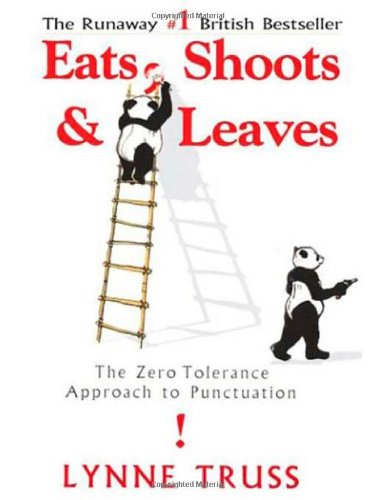
\includegraphics[width=0.5\textwidth]{images/eatshootsleaves.jpg}
\end{center}

\end{frame}

\begin{frame}
\frametitle{Revenge of English Class}

Grammatical correctness is a \textit{huge} issue in contracts. 

Here's a contract between Rogers Communications and Bell Aliant.

This did not go before the courts but before the CRTC\footnote{Canadian Radio-television\& Telecommunications Commission -- the telecom regulator} which ruled on it.


\end{frame}



\begin{frame}
\frametitle{The Original Text}

\begin{quote}
This agreement shall be effective from the date it is made and shall continue in force for a period of five (5) years from the date it is made, and thereafter for successive five (5) year terms, unless and until terminated by one year prior notice in writing by either party.
\end{quote}

Note that the term ``and thereafter for successive five (5) year terms'' is enclosed in commas and parenthetical - it can be removed from the sentence.

The unless and until clause can be then applied to the initial period.

\end{frame}



\begin{frame}
\frametitle{Two Interpretations}

Bell Aliant claimed the agreement should be interpreted like this:
 
\begin{quote}
{\color{red} This agreement shall be effective from the date it is made and shall continue in force for a period of five (5) years from the date it is made}, and thereafter for successive five (5) year terms, {\color{red} unless and until terminated by one year prior notice in writing by either party.}
\end{quote}

Rogers claimed it was intended to be like this:

\begin{quote}
{\color{red}
This agreement shall be effective from the date it is made and shall continue in force for a period of five (5) years from the date it is made,} {\color{blue} and thereafter for successive five (5) year terms unless and until terminated by one year prior notice in writing by either party.}
\end{quote}

Who won and why?

\end{frame}



\begin{frame}
\frametitle{Who Won}

The real answer is: nobody. 

The CRTC initially ruled in favour of the strict interpretation, believing the comma was there because it was meant to be there.

Rogers successfully argued that the French language version, which has equal standing  with the English, demonstrated that they were correct.

In spite of this, it was no real victory, because the CRTC did not have the authority to enforce the decision anyway~\cite{comma}.

\end{frame}




\begin{frame}
\frametitle{The Rule of \textit{Contra Proferentem}}

When an ambiguity appears in the language of the contract, precedent is that it is interpreted against the party that authored the term.

The rule is \textit{Contra Proferentem}: Latin for ``against the one bringing forth''.

This is often applied to take-it-or-leave-it type contracts (e.g., insurance, phone, internet, etc.) called ``contracts of adhesion''.

It is necessary to track who made what changes to an agreement before it is signed -- both sides may make (counter-)offers during negotiations.
\end{frame}


\begin{frame}
\frametitle{The Rule of \textit{Contra Proferentem}}

For this rule to be applied, these conditions must be satisfied:

\begin{enumerate}
	\item The clause in question must be found to be ambiguous\footnote{Disagreement about its meaning does not necessarily mean ambiguity!}.
	\item Neither interpretation is obviously significantly more reasonable.
	\item No liberal interpretation resolves the ambiguity\footnote{The parol evidence rule still applies!}.
\end{enumerate}

If ambiguity exists and cannot be resolved then the rule applies.

\end{frame}



\begin{frame}
\frametitle{Implied Terms}

Parties to a contract cannot foresee all things and there may be things that are forgotten or overlooked.

This is different from the examination of the meanings of express terms.

\alert{Implied terms} are those that the parties have not included in their agreement, but in the opinion of the court, reasonable persons would have included.

\end{frame}



\begin{frame}
\frametitle{The \textit{Moorcock}}

Consider the case of the \textit{Moorcock}, 1889.

The owner of the \textit{Moorcock} entered into a contract with the owner of a wharf to dock the ship.

When the tide went out, the hull hit a ridge which damaged the ship.

The contract made no provision for ensuring the ship's safety while docked.

Did the courts decide that implied terms about the safety of the ship existed?

\end{frame}



\begin{frame}
\frametitle{The \textit{Moorcock}}

The courts decided that had the parties considered the situation, they would have made provisions for this in the contract.

The judgement reads:

\begin{quote}
   In business transactions such as this, what the law desires to effect by the implication is to give such business efficacy to the transaction as must have been intended at all events by both parties who are business men; not to impose on one side all perils of the transaction, or to emancipate one side from all the chances of failure, but to make each party promise in law as much, at all events as it must have been in the contemplation of both parties that he should be responsible for in respect to those perils or chances.
\end{quote}


\end{frame}



\begin{frame}
\frametitle{Implied Terms}

This lead to the implication that a contract can have terms that are not explicitly written into the contract, but are implied by the nature of the contract.

\textit{Pigott Construction Co. Ltd v W.J. Crowe Ltd.}, 1961 established the guideline:

\begin{quote}
   I have for a long time understood that rule to be that the Court has no right to imply in a written contract any such stipulation, unless , on considering the terms of the contract in a reasonable and business manner, an implication necessarily arises that the parties must have intended that the suggested stipulation should exist.
\end{quote}

\end{frame}



\begin{frame}
\frametitle{Expansion of Implied Terms}

Further to this, in \textit{Markland Associates Ltd. v Lohnes}, 1973, the Nova Scotia Supreme Court ruled that a building contract has a number of implied terms:

\begin{itemize}
\item The work and materials would be of reasonable quality \& meet standards
\item The work was to be conducted in a normal manner
\item The final product would be usable and meet needs
\item The work would be done in reasonable time
\end{itemize}

It is not necessary to cover literally every eventuality in a contract.

\end{frame}



\begin{frame}
\frametitle{\textit{G. Ford Homes Ltd. v Draft Masonry (York) Co. Ltd.}}

\textit{G. Ford Homes Ltd. v Draft Masonry (York) Co. Ltd.}, 1983 

The subcontractor was in the business of fabricating and installing staircases.

The subcontractor offered the contractor a selection of possible options, of which, the contractor picked one.

The resulting installation it was 1.5" (3.81 cm) short on headspace...\\
\quad Violating the building code.

This required that the staircase be replaced.\\
\quad The contractor sought to recover the cost.

What did the court find in this case?

\end{frame}



\begin{frame}
\frametitle{\textit{G. Ford Homes Ltd. v Draft Masonry (York) Co. Ltd.}}

The subcontractor was found to be responsible for the cost of replacement.

The court found that the subcontractor was an ``expert'' and should have been aware of the Ontario Building Code.

It is reasonable to rely on the subcontractor to supply staircases that comply with the code.

Without the term there could be no business efficacy and to approve of the installation  would be tantamount to approval of an illegal contract~\cite{lpe}.

\end{frame}



\begin{frame}
\frametitle{\textit{Canadian Pacific Hotels Ltd. v. Bank of Montreal}, 1987}

The case involved a banking agreement between a hotel chain and its bank.

An employee of the hotel company wrote fraudulent cheques and forged signatures on them.

The bank normally required its customers to sign a ``verification agreement'': obliging the customer to check its bank statements and report discrepancies.

CP Hotels did not have such a term in their agreement with the bank.

The forgeries were discovered and CP Hotels wished to recover the fraudulently debited amounts from the bank.

Does there exist an implied term of the verification agreement?

\end{frame}


\begin{frame}
\frametitle{\textit{Canadian Pacific Hotels Ltd. v. Bank of Montreal}, 1987}

The bank argued they were not responsible.

Potential arguments supporting the bank's position include:\\
\quad (1) Verification is a usual term and would normally have been there.\\
\quad (2) It was the negligence of the customer that caused the customer's losses and the hotel chain had a responsibility to prevent its losses.

Potential arguments supporting the hotel chain include:\\
\quad (1) The bank and customer, equally capable of negotiating, came to an agreement without this term.\\
\quad (2) The courts should not create additional duties for the parties not found within existing law.

So: should the verification agreement be implied in the contract?

\end{frame}



\begin{frame}
\frametitle{\textit{Canadian Pacific Hotels Ltd. v. Bank of Montreal}, 1987}


The judgement reads:

\begin{quote}
A customer of a bank does not, in the absence of a verification agreement, owe a duty to the bank to examine bank statements with reasonable care and to report any discrepancies within a reasonable time, nor does a customer, ``sophisticated'' or otherwise, owe a duty to its bank to maintain an adequate system of internal accounting controls for the prevention and minimization of loss through forgery. There is no basis under any of the categories of implication for holding either duty to be an implied term of the contract between banker and customer.
\end{quote}

The bank, had it wished for the customer to be held to a verification agreement, ought to have included that as a term of the contract.

In its absence, the court will not declare one to be implicit.


\end{frame}


\begin{frame}
\frametitle{References \& Disclaimer}
\bibliographystyle{alphaurl}
\setbeamertemplate{bibliography item}{\insertbiblabel}
{\scriptsize
\bibliography{290}
}
\vfill

{\tiny Disclaimer: the material presented in these lectures slides is intended for use in the course ECE~290 at the University of Waterloo and should not be relied upon as legal advice. Any reliance on these course slides by any party for any other purpose are the responsibility of such parties.  The author(s) accept(s) no responsibility for damages, if any, suffered by any party as a result of decisions made or actions based on these course slides for any other purpose than that for which it was intended.\par}


\end{frame}


\end{document}

